\documentclass{article}



\usepackage{arxiv}

\usepackage[utf8]{inputenc} % allow utf-8 input
\usepackage[T1]{fontenc}    % use 8-bit T1 fonts
\usepackage{hyperref}       % hyperlinks
\usepackage{url}            % simple URL typesetting
\usepackage{booktabs}       % professional-quality tables
\usepackage{amsfonts}       % blackboard math symbols
\usepackage{nicefrac}       % compact symbols for 1/2, etc.
\usepackage{microtype}      % microtypography
\usepackage{lipsum}		% Can be removed after putting your text content
\usepackage{listings}
\usepackage{url}
\usepackage{graphicx}


\title{A MAST analysis of a Ravenscar application example}

%\date{September 9, 1985}	% Here you can change the date presented in the paper title
%\date{} 					% Or removing it

\author{
  Giovanni Jiayi Hu\\
  Department of Mathematics\\
  University of Padua, Italy I-35121\\
  \texttt{Email: giovannijiayi.hu@studenti.unipd.it} \\
  %% examples of more authors
   \And
   Alessio Gobbo \\
   Department of Mathematics\\
   University of Padua, Italy I-35121\\
   \texttt{Email: alessio.gobbo@studenti.unipd.it} \\
  %% \AND
  %% Coauthor \\
  %% Affiliation \\
  %% Address \\
  %% \texttt{email} \\
  %% \And
  %% Coauthor \\
  %% Affiliation \\
  %% Address \\
  %% \texttt{email} \\
  %% \And
  %% Coauthor \\
  %% Affiliation \\
  %% Address \\
  %% \texttt{email} \\
}

% Uncomment to remove the date
%\date{}

% Uncomment to override  the `A preprint' in the header
\renewcommand{\headeright}{Technical Report}
\renewcommand{\undertitle}{Technical Report}

\begin{document}
\maketitle

\begin{abstract}
Buchi del culo. \lipsum[1]
\end{abstract}


% keywords can be removed
% \keywords{First keyword \and Second keyword \and More}

\section{Introduction}

There is increasing recognition that the software components of critical real-time applications must be provably predictable. This is particularly so for a hard real-time system, in which the failure of a component of the system to meet its timing deadline can result in an unacceptable failure of the whole system. The choice of a suitable design and development method, in conjunction with supporting tools that enable the real-time performance of a system to be analysed and simulated, can lead to a high level of confidence that the final system meets its real-time constraints.

The use of Ada has proven to be of great value within high integrity and real-time applications, albeit via language subsets of deterministic constructs, to ensure full analysability of the code. The research work in schedulability analysis has been mapped onto a number of new Ada constructs and rules that have been incorporated into the Real-Time Annex of the Ada language standard [RM D]. This has opened the way for these tasking constructs to be used in high integrity subsets whilst retaining the core elements of predictability and reliability.

The Ravenscar Profile is a subset of the tasking model, restricted to meet the real-time community requirements for determinism, schedulability analysis and memory-boundedness, as well as being suitable for mapping to a small and efficient run-time system that supports task synchronization and communication, and which could be certifiable to the highest integrity levels.

The example presented in this paper is extracted from "Guide for the use of the
Ada Ravenscar Profile in
high integrity systems" \cite{ycs} and it is designed to illustrate the expressive power of the Ravenscar Profile and the associated coding paradigms, which aim to facilitate off-line scheduling analysis.

The extended application example uses all of the concurrency components permitted by the Ravenscar Profile. The structure of the example models, on a reduced and simplified scale, the operation of real-world embedded real-time systems.

The example system includes a periodic process that handles orders for a variable amount of workload. Whenever the request level exceeds a certain threshold, the periodic process farms the excess load out to a supporting sporadic process. While such orders are executed, the system may receive interrupt requests from an external source. Each interrupt treatment records an entry in an activation log. When specific conditions hold, the periodic process releases a further sporadic process to perform a check on the interrupt activation entries recorded in the intervening period. The policy of work delegation adopted by the system allows the periodic process to ensure the constant discharge of a guaranteed level of workload. The correct implementation of this policy also requires assigning the periodic process a higher priority than those assigned to the sporadic processes, so that guaranteed work can be performed in preference to subsidiary activities.

MAST, a Modeling and Analysis Suite for Real-Time Applications, is a model for representing the temporal and logical elements of real-time applications \cite{mast}. This model allows a very rich description of the system, including the effects of event or message-based synchronization, multiprocessor and distributed architectures as well as shared resource synchronization.

MAST offers a graphical user interface but it's still immature to be completely usable. Too many frequent bugs.

\section{Board STM32F429I-Discovery}

We have preferred the usage of a bare-board instead of the GNAT emulator because the measure time values had too much standard deviation.

It has ST-LINK debugger built-in.

\section{Execution times}

Execution times are measured using two packages \texttt{System\_Overhead} and \texttt{Task\_Overhead}.

\section{MAST Model}

For a reference to the MAST syntax, visit "Description of the MAST Model" \cite{mast-description}. Since we are dealing with hard real-time analysis, we define only the WCET to the operations. Anyway most of the time, except for the Whetstone operations, we had deterministic execution times with always the same number of CPU ticks or with a difference less than 1micros.

\begin{lstlisting}
Processing_Resource (
   Type                   => Regular_Processor,
   Name                   => cpu,
   Max_Interrupt_Priority => 255,
   Min_Interrupt_Priority => 241,
   Worst_ISR_Switch       => 2.578E-06,
   System_Timer           =>
      ( Type           => Ticker,
        Worst_Overhead => 3.844E-06,
        Period         => 0.001000),
   Speed_Factor           => 1.00);
\end{lstlisting}

We have a board with only one CPU and interrupt ranges are taken from \texttt{System} package. Task priorities range from 1 to 240, whereas interrupt priorities go from 241 to 255. So we have at maximum 240 task priorities, if we ever would need more priorities we could use the technique described in \cite{limited-priorities}. The Interrupt Service Routine overhead is measured as the time taken to execute \texttt{Interrupt\_Handler} in \texttt{System.BB.Board\_Support} package, apart from the execution time of the user-defined interrupt handler. It takes into account the overhead of managing the Task and Interrupt Execution Clocks \cite{etc}.

The system timer used by the board is Tick Scheduling \cite{tick-scheduling}, which is accounted in the analysis using the technique described in \cite{effects-runtime}. The period of the tick is 1ms, as defined in \texttt{System.BB.Board\_Support} package, and the worst overhead is measured as the time taken to execute \texttt{Timer\_Interrupt\_Handler}, the trap handler defined in the same package for \texttt{Sys\_Tick} trap.

\begin{lstlisting}
Scheduler (
   Type            => Primary_Scheduler,
   Name            => fps,
   Host            => cpu,
   Policy          =>
      ( Type                 => Fixed_Priority,
        Worst_Context_Switch => 3.090E-06,
        Max_Priority         => 240,
        Min_Priority         => 1));
\end{lstlisting}

We only have one primary scheduler in the system, no hierarchical scheduling. The context switch overhead is measured as time to trigger the context switch interrupt \texttt{Pend\_SV} and the execution time of \texttt{Pend\_SV\_Handler} in \texttt{System.BB.CPU\_Primitives.Context\_Switch\_Trigger} package, to save the active context and load the new one.

\begin{lstlisting}
Scheduling_Server (
   Type                       => Regular,
   Name                       => regular_producer,
   Server_Sched_Parameters    =>
      ( Type         => Fixed_Priority_Policy,
        The_Priority => 7,
        Preassigned  => YES),
   Scheduler                  => fps);

Scheduling_Server (
   Type                       => Regular,
   Name                       => on_call_producer,
   Server_Sched_Parameters    =>
      ( Type         => Fixed_Priority_Policy,
        The_Priority => 5,
        Preassigned  => YES),
   Scheduler                  => fps);

Scheduling_Server (
   Type                       => Regular,
   Name                       => activation_log_reader,
   Server_Sched_Parameters    =>
      ( Type         => Fixed_Priority_Policy,
        The_Priority => 3,
        Preassigned  => YES),
   Scheduler                  => fps);

Scheduling_Server (
   Type                       => Regular,
   Name                       => external_event_server,
   Server_Sched_Parameters    =>
      ( Type         => Fixed_Priority_Policy,
        The_Priority => 11,
        Preassigned  => YES),
   Scheduler                  => fps);

Scheduling_Server (
   Type                       => Regular,
   Name                       => interrupt_server,
   Server_Sched_Parameters    =>
      ( Type         => Interrupt_FP_Policy,
        The_Priority => 241),
   Scheduler                  => fps);
\end{lstlisting}

Each task is a Scheduling Server, whereas \texttt{interrupt\_server} models the runtime which runs the Interrupt Service Routine using the technique described in \cite{interrupt-handler}.

\begin{lstlisting}
Shared_Resource (
   Type        => Immediate_Ceiling_Resource,
   Name        => request_buffer,
   Ceiling     => 9,
   Preassigned => YES);

Shared_Resource (
   Type        => Immediate_Ceiling_Resource,
   Name        => activation_log,
   Ceiling     => 13,
   Preassigned => YES);

Shared_Resource (
   Type        => Immediate_Ceiling_Resource,
   Name        => event_queue,
   Ceiling     => 241,
   Preassigned => YES);
\end{lstlisting}

Protected objects are modeled as Shared Resourses which use the Immediate Priority Ceiling Protocol, the same defined as \texttt{Priority Ceiling Locking} in Ada Reference Manual D.3.

\begin{lstlisting}
Operation (
   Type                       => Simple,
   Name                       => rb_deposit,
   Worst_Case_Execution_Time  => 2.000E-06,
   Shared_Resources_To_Lock   =>
      ( request_buffer),
   Shared_Resources_To_Unlock =>
      ( request_buffer));

Operation (
   Type                       => Simple,
   Name                       => rb_extract,
   Worst_Case_Execution_Time  => 2.000E-06,
   Shared_Resources_To_Lock   =>
      ( request_buffer),
   Shared_Resources_To_Unlock =>
      ( request_buffer));
\end{lstlisting}

Protected methods are modeled as simple operations which lock and unlock the protected object resourse. The execution time is measured from the first line of the method to the last one, so it doesn't include the runtime overhead associated with invoking protected methods.

\begin{lstlisting}
Operation (
   Type                     => Enclosing,
   Name                     => ocp_start,
   Worst_Case_Execution_Time=> 6.000E-06,
   Composite_Operation_List =>
      ( rb_deposit));

Operation (
   Type                     => Enclosing,
   Name                     => rb_extract_enclosing,
   Worst_Case_Execution_Time=> 7.000E-06,
   Composite_Operation_List =>
      ( rb_extract));
\end{lstlisting}

For each protected method there is an Enclosing operation which takes into account the overhead associated with invoking protected methods. Sometimes it's already a method defined by GEE, other times it's defined in the model on purpose. By doing so we can define the more complex methods as Composite operations, which have the execution time as the sum of the execution times of the comprised operations.

\begin{lstlisting}
Operation (
   Type                       => Simple,
   Name                       => rp_small_whetstone,
   Worst_Case_Execution_Time  => 0.019363);

Operation (
   Type                     => Composite,
   Name                     => rp_operation,
   Composite_Operation_List =>
      ( rp_small_whetstone,
        due_activation,
        ocp_start,
        check_due,
        alr_signal,
        put_line));

Operation (
   Type                     => Composite,
   Name                     => regular_producer,
   Composite_Operation_List =>
      ( overrun_detection,
        rp_operation,
        delay_until));
\end{lstlisting}

Therefore, by changing the worload parameter of \texttt{Small\_Whetstone} in the application implementation, we will be able to test different utilisation of the system with likewise ease in updating the MAST model. The Whetstone execution time is proportional to the workload parameter. If we wanted to try what happens by increasing the load of factor 10, we would just increase the WCET to \texttt{0.19363}, without the need to measure again all the Enclosing operations, since all the methods which use the Whetstone are defined as Composite. However we have been careful to avoid forgetting any overhead in a Composite method and make sure they are not impacted by any change of the Whetstone workload. For instance, if we had defined \texttt{regular\_producer} as Enclosing we could have defined as composed of only \texttt{rp\_operation} and then measure its WCET, which will implicitly count also overrun detection and delay queue overhead. By instead defining it as Composite, we have been careful to define the simple operations \texttt{overrun\_detection} and \texttt{delay\_until} to include their execution time, using the technique described in \cite{effects-runtime}.

\begin{lstlisting}
Transaction (
   Type            => regular,
   Name            => rp_transaction,
   External_Events =>
      ( ( Type       => Periodic,
          Name       => e1,
          Period     => 1.000,
          Max_Jitter => 0.000,
          Phase      => 0.000)),
   Internal_Events =>
      ( ( Type => Regular,
          Name => rpo1,
          Timing_Requirements =>
            ( Type             => Hard_Global_Deadline,
              Deadline         => 0.500000,
              Referenced_Event => e1))),
   Event_Handlers  =>
      ( (Type               => System_Timed_Activity,
         Input_Event        => e1,
         Output_Event       => rpo1,
         Activity_Operation => regular_producer,
         Activity_Server    => regular_producer)));
\end{lstlisting}

The main event stream is modeled as a transaction activated by a periodic external event, with period of 1s. The event is handled by the \texttt{regular\_producer} operation by the task of the same name. The Event Handler is of type \texttt{System\_Timed\_Activity} to take into account the jitter and the overhead caused by the tick scheduling

\begin{lstlisting}
Transaction (
   Type            => regular,
   Name            => ocp_transaction,
   External_Events =>
      ( ( Type             => Sporadic,
          Name             => ocp_activation,
          Avg_Interarrival => 5.000,
          Distribution     => UNIFORM,
          Min_Interarrival => 5.000)),
   Internal_Events =>
      ( ( Type => Regular,
          Name => ocpo1,
          Timing_Requirements =>
            ( Type             => Hard_Global_Deadline,
              Deadline         => 0.800000,
              Referenced_Event => ocp_activation))),
   Event_Handlers  =>
      ( (Type               => Activity,
         Input_Event        => ocp_activation,
         Output_Event       => ocpo1,
         Activity_Operation => on_call_producer,
         Activity_Server    => on_call_producer)));
\end{lstlisting}

The sporadic \texttt{On Call Producer} event stream is modeled as activated by a bounded aperiodic event, with minimum interarrival time of 5s and uniform distribution. Actually we know that the interarrival time is precisely 5s, thus the same value as average interarrival. Similar modeling has been done for the \texttt{Activation Log Reader} sporadic task.

\begin{lstlisting}
Transaction (
   Type            => regular,
   Name            => event_queue_interrupt,
   External_Events =>
      ( ( Type             => Sporadic,
          Name             => button_click,
          Avg_Interarrival => 0.000,
          Distribution     => UNIFORM,
          Min_Interarrival => 5.000)),
   Internal_Events =>
      ( ( Type => Regular,
          Name => eqo1),
        ( Type => Regular,
          Name => eqo2,
          Timing_Requirements =>
            ( Type             => Hard_Global_Deadline,
              Deadline         => 0.100000,
              Referenced_Event => button_click))),
   Event_Handlers  =>
      ( (Type               => Activity,
         Input_Event        => button_click,
         Output_Event       => eqo1,
         Activity_Operation => eq_signal,
         Activity_Server    => interrupt_server),
        (Type               => Activity,
         Input_Event        => eqo1,
         Output_Event       => eqo2,
         Activity_Operation => external_event_server,
         Activity_Server    => external_event_server)));
\end{lstlisting}

The blue button interrupt event stream is modeled as a triggered by a sporadic event of 5s as minimum interarrival time and it's first handled by the \texttt{interrupt\_server} which runs the ISR at interrupt priority level and then by the user-defined \texttt{external\_event\_server} at task priority-level.

\section{Overrun detection}

\begin{lstlisting}[language=Ada]
-- Overrun.ads

with Ada.Real_Time;
with Ada.Execution_Time;

package Overrun is
   type Limits_Array is array (0 .. 2) of Ada.Execution_Time.CPU_Time;

   procedure Start (Index : Natural; Budget : Ada.Real_Time.Time_Span);
   procedure Check (Index : Natural);
end Overrun;
\end{lstlisting}

\begin{lstlisting}[language=Ada]
-- Overrun.adb

with Ada.Real_Time; use Ada.Real_Time;
with Ada.Execution_Time; use Ada.Execution_Time;

package body Overrun is
   use Ada.Real_Time;
   use Ada.Execution_Time;

   Limits : Limits_Array := (CPU_Time_First, CPU_Time_First, CPU_Time_First);

   procedure Start (Index : Natural; Budget : Time_Span) is
   begin
      Limits (Index) := Ada.Execution_Time.Clock + Budget;
   end Start;

   procedure Check (Index : Natural) is
   begin
      if Ada.Execution_Time.Clock > Limits (Index) then
         raise Program_Error with "Detected overrun";
      end if;
   end Check;
end Overrun;
\end{lstlisting}

Ispiration from \cite{overrundetection}. The measured execution times include overrun detection overhead for Regular Producer, On Call Producer and Activation Log Reader.

\section{MAST analysis}

As of the time of writing, MAST is at version 1.5.1 and supports the following analysis tools.

\begin{figure}[!htbp]
\centering
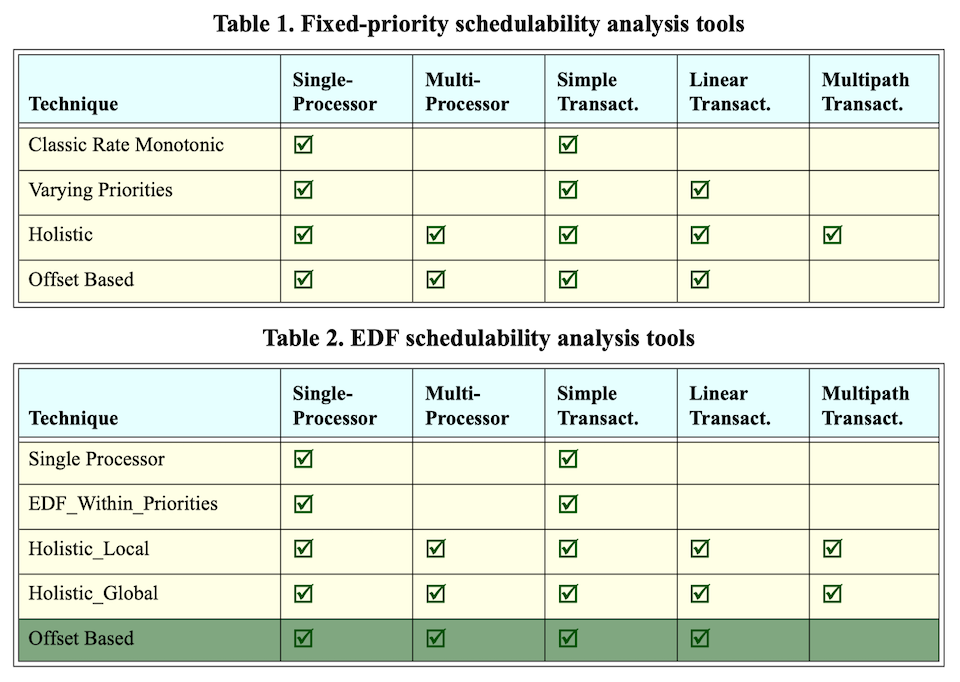
\includegraphics[width=5in]{images/mast-analysis}
\caption{MAST analysis tools \cite{mast-description}.}
\label{mast-analysis-tools}
\end{figure}

The transaction which defines the button interrupt event stream is considered as a linear transaction, which only has one external event and that its Event handlers are all Activities, but unfortunately it is not a simple transaction, a continuous sequence of activities executed by the same server. We have one server which handles the ISR and another one the associated task of External Event Server.

This means we cannot use the classic Rate Monotonic algorithm \cite{rm-dm}, only offset-based (cite ?) and holistic analysis \cite{holistic-analysis}. We decided to stick to only holistic analysis because it supports both FPS and EDF, whereas offset-based fallbacks to holistic analysis with EDF processing resources \cite{mast-readme}. Nevertheless it doesn't make much difference which one is used between holistic and offset-based since we run the system on a single processor, not on a distributed system (?).

\subsection{Holistic analysis}

In our application we have chains of operations, not independent tasks competing for the shared resourses. The technique described in \cite{practitioner-common-data} assumes the worst case, but it's too pessimist because in our case a task A always precedes task B, they are not independent and competing for the same resourses. Therefore we use the holistic analysis, designed originally for distributed systems.

\section{FPS analysis}

\begin{table}[!htbp]
  \centering
  \begin{tabular}{llll}
    \toprule
    Transaction & Worst case response time (s) & Slack & Worst blocking time (s)  \\
    \midrule
    rp\_transaction & 0.020393  & 2477.0\% &  2.000E-06  \\
    ocp\_transaction & 0.026525 & 10852.0\% & 1.000E-06 \\
    alr\_transaction & 0.030109 & 27088.7\% & 0.00 \\
    event\_queue\_interrupt & 3.818E-05 & N/A & 1.000E-06 \\
    \bottomrule
  \end{tabular}
  \caption{Holistic analysis results for FPS}
  \label{tab:holistic-fps}
\end{table}

The system slack is 2401.2\% and total utilisation 2.59\%.

We then increase the Whetstone workload of factor 24 in the first three transactions since 2477.0\% is the smallest slack of three transactions. We leave the Event Queue interrupt unchanged. The new results are as follows:

\begin{table}[!htbp]
   \centering
   \begin{tabular}{llll}
     \toprule
     Transaction & Worst case response time (s) & Slack & Worst blocking time (s)  \\
     \midrule
     rp\_transaction & 0.487017  & 2.34\% &  2.000E-06  \\
     ocp\_transaction & 0.664777 & 75.39\% & 1.000E-06 \\
     alr\_transaction & 0.754207 & 273.44\% & 0.00 \\
     event\_queue\_interrupt & 3.818E-05 & >=100000.0\% & 1.000E-06 \\
     \bottomrule
   \end{tabular}
   \caption{Holistic analysis results for FPS}
   \label{tab:holistic-fps}
\end{table}

Blocking times have not changed because protected operations are same as before.

The system slack is 2.80\% and total utilisation 55.33\%. The theoretical CPU utilisation upper bound \cite{liu-utilisation-bound} is 0.779 for tasks with same deadline as the period, but we have to use the technique shown in \cite{practitioner-utilisation-bound}. We now increase the workloads of factor 25 instead of 24\%.

\begin{table}[!htbp]
   \centering
   \begin{tabular}{llll}
     \toprule
     Transaction & Worst case response time (s) & Slack & Worst blocking time (s)  \\
     \midrule
     rp\_transaction & 0.506453  & -1.56\% &  2.000E-06  \\
     ocp\_transaction & 0.691366 & -100.00\% & 1.000E-06 \\
     alr\_transaction & 0.784369 & -100.00\% & 0.00 \\
     event\_queue\_interrupt & 3.818E-05 & -100.00\% & 1.000E-06 \\
     \bottomrule
   \end{tabular}
   \caption{Holistic analysis results for FPS}
   \label{tab:holistic-fps}
\end{table}

The system slack is -1.16\% and total utilisation 57.53\%, which exceed the theoretical limit (?). This means that the actual execution should also overrun the deadline and it is indeed what happened on our board. The first job of Regular Producer raised the overrun detection Program Error.

\bibliographystyle{unsrt}
%\bibliography{references}  %%% Remove comment to use the external .bib file (using bibtex).
%%% and comment out the ``thebibliography'' section.


%%% Comment out this section when you \bibliography{references} is enabled.
\begin{thebibliography}{1}

\bibitem{ycs}
A Burns, B Dobbing, T Vardanega.
\newblock Guide for the use of the Ada Ravenscar Profile in high integrity systems.
\newblock In {\em University of York Technical Report YCS-2003-348}. January 2003.

\bibitem{mast}
M. GonzAlez Harbour, J.J. GutiCrrez Garcia, J.C. Palencia GutiCrrez, and J.M. Drake Moyano.
\newblock MAST Modeling and Analysis Suite for Real Time Applications.
\newblock In {\em Proceedings 13th Euromicro Conference on Real-Time Systems}. 2001.

\bibitem{mast-description}
J. M. Drake, M. G. Harbour, J. J. Gutiérrez, P. L. Martínez, J. L. Medina, J. C. Palencia
\newblock Description of the MAST Model.
\newblock \url{https://mast.unican.es/mast_description.pdf}

\bibitem{mast-readme}
J. M. Drake, M. G. Harbour, J. J. Gutiérrez, P. L. Martínez, J. L. Medina, J. C. Palencia
\newblock MAST README.
\newblock \url{https://mast.unican.es/README.txt}

\bibitem{overrundetection}
Juan Zamorano, Alejandro Alonso, José Antonio Pulido, Juan Antonio de la Puente.
\newblock Implementing Execution-Time Clocks for the Ada Ravenscar Profile.
\newblock In {\em Reliable Software Technologies - Ada-Europe 2004}. pp 132-143. Ada-Europe 2004.

\bibitem{rm-dm}
Jane W. S. W. Liu.
\newblock Rate-Monotonic and Deadline-Monotonic Algorithms.
\newblock In {\em Real-Time Systems}. pp 118-119. 2001.

\bibitem{limited-priorities}
Jane W. S. W. Liu.
\newblock Limited-Priority Levels.
\newblock In {\em Real-Time Systems}. pp 166-168. 2001.

\bibitem{tick-scheduling}
Jane W. S. W. Liu.
\newblock Tick Scheduling.
\newblock In {\em Real-Time Systems}. pp 168-171. 2001.

\bibitem{holistic-analysis}
KenTindell, JohnClark.
\newblock Holistic schedulability analysis for distributed hard real-time systems.
\newblock In {\em Microprocessing and Microprogramming}. Volume 40, Issues 2–3, pp 117-134. April 1994.

\bibitem{liu-utilisation-bound}
C. L. Liu, James W. Layland.
\newblock Scheduling Algorithms for Multiprogramming in a Hard-Real-Time Environment.
\newblock In {\em Journal of the ACM}. Volume 20 Issue 1, pp 46-61. Jan. 1973.

\bibitem{practitioner-utilisation-bound}
Klein, M., Ralya, Th., Pollak, B., Obenza, R., Harbour, M.G. .
\newblock Using Utilization Bounds for Each Event when Deadlines Are Within the Period.
\newblock In {\em A Practitioner’s Handbook for Real-Time Analysis
}. chapter 4.1.2. 1993.

\bibitem{practitioner-common-data}
Klein, M., Ralya, Th., Pollak, B., Obenza, R., Harbour, M.G. .
\newblock Designing Tasks that Must Synchronize to Share Common Data.
\newblock In {\em A Practitioner’s Handbook for Real-Time Analysis
}. chapter 5.2. 1993.

\bibitem{effects-runtime}
Klein, M., Ralya, Th., Pollak, B., Obenza, R., Harbour, M.G. .
\newblock Effects of Operating System and Runtime Services on Timing Analysis.
\newblock In {\em A Practitioner’s Handbook for Real-Time Analysis
}. chapter 7. 1993.

\bibitem{interrupt-handler}
Klein, M., Ralya, Th., Pollak, B., Obenza, R., Harbour, M.G. .
\newblock Use an Interrupt Handler.
\newblock In {\em A Practitioner’s Handbook for Real-Time Analysis
}. chapter 5.3.5.1. 1993.

\bibitem{etc}
Kristoffer Nyborg Gregertsen, Amund Skavhaug.
\newblock Implementation and Usage of the new Ada 2012 Execution Time Control Features.
\newblock In {\em Ada User Journal}. 2011.

\end{thebibliography}


\end{document}
